\SourceLeaf{632}
\[
\begin{aligned}
\omega X&=\frac{\varepsilon ik\zeta\omega}{r^5}\left\{3xy\left(\frac{\mathrm dz}{\mathrm dx}\right)+(2rr-3xx-3zz)\left(\frac{\mathrm dz}{\mathrm dy}\right)-3yz\right\}\\
&=\frac{\varepsilon ik\zeta\omega}{r^5}\Big\{\left(x\frac{\mathrm ddz}{\mathrm dx\mathrm dy}+\frac{\mathrm dz}{\mathrm dy}\right)rr-3\left(x+z\frac{\mathrm dz}{\mathrm dx}\right)x\frac{\mathrm dz}{\mathrm dy}\\
&\quad-\left(x\frac{\mathrm ddz}{\mathrm dx\mathrm dy}-\frac{\mathrm dz}{\mathrm dy}\right)rr+3\left(y+z\frac{\mathrm dz}{\mathrm dy}\right)\left(x\frac{\mathrm dz}{\mathrm dx}-z\right)\Big\}\\
&=\varepsilon ik\zeta\omega\left\{\frac{\mathrm d\dfrac{x\left(\frac{\mathrm dz}{\mathrm dy}\right)}{r^3}}{\mathrm dx}-\frac{\mathrm d\dfrac{x\left(\frac{\mathrm dz}{\mathrm dx}\right)-z}{r^3}}{\mathrm dy}\right\}
\end{aligned}
\]

Soll nun die Totalwirkung parallel mit der Axe der $x$ ermittelt werden, so nennen wir III die Projection von I auf die Ebene der $x,y$ oder den Inbegriff aller $\omega$ und haben mithin das Integral $\int\omega X$ über alle $\omega$ ausgedehnt aufzusuchen, oder wenn wir $\mathrm dx\mathrm dy$ anstatt $\omega$ schreiben, haben wir die doppelte Integration von $X\mathrm dx\mathrm dy$ auszuführen.

Man hat hiebei
\[
\varepsilon ik\zeta\mathrm dy.\left\{\frac{\mathrm d\dfrac{x\left(\frac{\mathrm dz}{\mathrm dy}\right)}{r^3}}{\mathrm dx}.\mathrm dx\right\}
\]
und
\[
\varepsilon ik\zeta\mathrm dx.\left\{\frac{\mathrm d\dfrac{x\left(\frac{\mathrm dz}{\mathrm dx}\right)-z}{r^3}}{\mathrm dy}.\mathrm dy\right\}
\]
besonders zu betrachten. Für ersteres theilt man III in unendlich viele unendlich schmale Streifen parallel mit der Axe der $x$, für zweites in ähnliche Streifen, aber parallel mit der Axe der $y$. Daraus folgt dann sehr leicht, dass das Ganze wird
\[
\varepsilon ik\zeta\int\frac{x\mathrm dz-z\mathrm dx}{r^3}=\varepsilon ik\zeta\int\frac{x\dfrac{\mathrm dz}{\mathrm ds}-z\dfrac{\mathrm dx}{\mathrm ds}}{r^3}.\mathrm ds
\]
durch den ganzen Umfang von III ausgedehnt, indem man diesen in einer solchen Richtung durchläuft, dass III rechts liegt.

Auf ähnliche Weise erhält man für die Summe aller $Y\omega$
\[
\varepsilon ik\zeta\int\frac{y\mathrm dz-z\mathrm dy}{r^3}=\varepsilon ik\zeta\int\frac{y\dfrac{\mathrm dz}{\mathrm ds}-z\dfrac{\mathrm dy}{\mathrm ds}}{r^3}.\mathrm ds
\]
Hiedurch in Verbindung mit [Nr. 14] ist das \textsc{Ampère}sche Gesetz bewiesen.

\SourceLeaf{633}
\begin{center}[20]\par\medskip[\textit{C. F. Gauss an W. Weber.}]\end{center}
Hoch geschätzter Freund.

Seit Anfang dieses Jahrs ist unaufhörlich auf so vielfache Weise meine Zeit in Anspruch genommen und zersplittert, und von der andern Seite mein Gesundheitszustand anhaltenden Arbeiten so wenig günstig gewesen, dass ich bisher gar nicht habe dazu kommen können, den mir von Ihnen gütigst vor zwei Monaten zugesandten kleinen Aufsatz durchzugehen, und dass ich erst jetzt eine flüchtige Durchsicht habe vornehmen können. Diese hat mir aber gezeigt, dass der Gegenstand zu denselben Untersuchungen gehört, mit denen ich mich vor etwa 10 Jahren (ich meine besonders 1834—1836) sehr ausgedehnt beschäftigt habe, und dass um ein gründliches und erschöpfendes Urtheil über Ihren Aufsatz aussprechen zu können, es nicht zureicht \textit{diesen} durchzulesen, sondern dass ich mich erst ganz wieder in meine eignen Arbeiten aus jener Zeit würde hineinstudiren müssen, was einen um so längern Zeitraum erfordern würde, da ich jetzt, bei einer versuchsweise vorgenommenen Papier-Durchmusterung erst einige nur fragmentarische Bruchstücke aufgefunden habe, obwohl wahrscheinlich viel mehr noch vorhanden sein wird, wenn auch nicht in vollständig geordneter Form.

Darf ich aber, jenen Gegenständen seit mehreren Jahren entfremdet, auf den Grund des Gedächtnisses eine Urtheilsäusserung mir verstatten, so würde ich glauben, dass von vorne herein \textsc{Ampère}, lebte er noch, entschieden dagegen protestiren würde, wenn Sie das \textsc{Ampère}sche Fundamentalgesetz durch die Formel
\[
-\frac{\alpha\alpha'}{rr}ii'\sin\theta\sin\theta'\cos\varepsilon\tag*{(I)}
\]
ausdrücken, da jenes ein ganz davon verschiedenes nemlich in der Formel
\[
-\frac{\alpha\alpha'}{rr}ii'\left(\tfrac12\cos\theta\cos\theta'+\sin\theta\sin\theta'\cos\varepsilon\right)\tag*{(II)}
\]
enthaltenes ist. Ich glaube auch nicht, dass \textsc{Ampère} durch die Zusatznote, deren Sie in einem spätern Briefe erwähnen, befriedigt sein würde, wo Sie nemlich den Unterschied so einkleiden, dass \textsc{Ampères} Formel eine \textit{allgemeinere} sei, eben wie $-\dfrac{\alpha\alpha'}{rr}(F\cos\theta\cos\theta'+G\sin\theta\sin\theta'\cos\varepsilon)$. wo \textsc{Ampère} aus Versuchen $F=\tfrac12G$ abgeleitet habe, während Sie, weil \textsc{Ampères} Versuche nicht sehr scharf seien, mit demselben Rechte den Werth $F=0$ in Anspruch nehmen zu können glauben. In jedem andern Falle, als dem vorliegenden, würde ich zugeben, dass ein dritter bei dieser Discordanz zwischen Ihnen und \textsc{Ampère} sich etwa so erklärte:

\SourceLeaf{634}
ob man (mit Ihnen) dies nur als eine Modification des \textsc{Ampère}schen Gesetzes ansehen, oder

ob (wie meines Erachtens \textsc{Ampère} die Sache würde ansehen müssen) dies ebenso viel heisse als ein completer Umsturz der \textsc{Ampère}schen Fundamentalformel und das Einsetzen einer wesentlich andern

sei doch im Grunde wenig mehr als ein müssiger Wortstreit. Wie gesagt, in jedem andern Fall würde ich dies gern einräumen, da niemand \textit{in verbis facilior} als ich sein kann. Aber in gegenwärtigem ist der Unterschied eine Lebensfrage, denn die ganze \textsc{Ampère}sche Theorie der Umtauschbarkeit des Magnetismus mit galvanischen Strömen hängt durchaus von der Richtigkeit der Formel II ab und geht gänzlich verloren, wenn eine andere dafür gewählt würde.

Ich kann Ihnen nicht widersprechen, wenn Sie die Versuche von \textsc{Ampère} für nicht sehr concludent erklären, zumal, da ich \textsc{Ampères} classische Abhandlung nicht zur Hand und die Art seiner Versuche gar nicht im Gedächtniss habe, indessen glaube ich doch nicht, dass \textsc{Ampère}, auch wenn er die Unvollkommenheit seiner Versuche selbst einräumte, die Befugniss, eine ganz andere Formel (I), wodurch seine ganze Theorie zerfiele, zu adoptiren zugeben würde, so lange nicht diese andere Formel durch \textit{ganz entscheidende} Versuche befestigt wäre. Die Bedenken, die ich selbst Ihrem zweiten Briefe zufolge, geäussert habe, müssen von Ihnen misverstanden sein. Ich habe früh die Überzeugung gewonnen und festgehalten, dass die oben erwähnte Vertauschbarkeit \textit{nothwendig} die \textsc{Ampère}sche Formel II erfordert und keine andere zulässt, die nicht mit jener, für einen geschlossenen Strom identisch wird, \textit{wenn die Wirkung in der Richtung der die beiden Stromelemente verbindenden geraden Linie} geschehen soll, dass man aber allerdings unzählige andere Formen wählen kann, wenn man die eben ausgesprochene Bedingung verlässt, die aber für einen geschlossenen Strom immer dasselbe Endresultat geben müssen wie \textsc{Ampères} Formel. Man könnte übrigens auch noch hinzufügen, dass da es bei jenen Zwecken immer nur um Wirkungen in messbaren Entfernungen sich handelt, nichts uns hindern würde, vorauszusetzen, dass auch noch möglicherweise andere Theile zu der Formel hinzukommen mögen, die nur in unmessbar kleinen Entfernungen wirksam sind (wie die Molecularattraction zu der Gravitation hinzutritt), und dass dadurch die Schwierigkeit des Abstossens zweier auf einander folgenden Elemente desselben Stromes beseitigt werden könnte.

\SourceLeaf{635}
Um Missverständniss zu verhüten; will ich noch bemerken, dass die obige Formel II auch so geschrieben werden kann
\[
-\frac{\alpha\alpha'}{rr}ii'\left(-\tfrac12\cos\theta\cos\theta'+\sin\theta\sin\theta'\cos\varepsilon\right)
\]
und dass ich nicht weiss, ob \textsc{Ampère} (dessen Memoire ich wie gesagt nicht zur Hand habe) die erste oder zweite Schreibart gebraucht hat. Beide bedeuten nemlich dasselbe, und man schreibt die erste Form, wenn man die Winkel $\theta$, $\theta'$ mit derselben (begrenzten) geraden Linie misst, also diese Linie bei dem zweiten Winkel im entgegengesetzten Sinn zum Schenkel wählt; die andere Form hingegen, wenn man eine gerade Linie von unbestimmter Länge betrachtet und zur Messung der Winkel $\theta$, $\theta'$, jene Linie beidemal in einerlei Sinn zuzieht. Und ebenso kann man der ganzen Formel anstatt des $-$ Zeichens ein $+$ Zeichen vorsetzen, wenn man nicht Abstossung sondern Anziehung wie eine positive Wirkung betrachtet.

Vielleicht bin ich im Stande, mich etwas mehr wieder in diese mir jetzt so fremd gewordenen Sachen hineinzustudiren, bis Sie, wie Sie mir Hoffnung gemacht haben Ende April oder Anfang Mai mich mit einem Besuche erfreuen. Ich würde ohne Zweifel meine Untersuchungen längst bekannt gemacht haben, hätte nicht zu der Zeit, wo ich sie abbrach, das gefehlt, was ich wie den eigentlichen Schlussstein betrachtet hatte
\begin{center}\textit{Nil actum reputans si quid superesset agendum}\end{center}
nemlich \textit{die Ableitung} der Zusatzkräfte (die zu der gegenseitigen Wirkung ruhender Electricitätstheile noch hinzukommen, wenn sie in gegenseitiger Bewegung sind) \textit{aus der nicht instantanen}, sondern (auf ähnliche Weise wie beim Licht) in der Zeit sich fortpflanzenden Wirkung. Mir hatte dies damals nicht gelingen wollen; ich verliess aber so viel ich mich erinnere die Untersuchung damals doch nicht ganz ohne Hoffnung, dass dies später vielleicht gelingen könnte, obwohl — erinnere ich mich recht — mit der subjectiven Überzeugung, dass es vorher nöthig sei, sich von der Art, \textit{wie} die Fortpflanzung geschieht, eine construirbare Vorstellung zu machen.
\begin{center}—\quad —\quad —\quad —\quad —\quad —\quad —\quad —\quad —\quad —\quad —\quad —\quad —\quad —\quad —\quad —\end{center}
\noindent\begin{minipage}{\linewidth}
Unter herzlichen Grüssen an Ihre Geschwister und an Herrn Prof. \textsc{Möbius}

Göttingen, 19. März 1845.\hfill stets der Ihrige
\begin{flushright}C. F. \textsc{Gauss}.\end{flushright}
\end{minipage}

\SourceLeaf{636}
\begin{center}[21.]\end{center}
\noindent Lineargrösse $=$ Widerstand eines gegebenen Drahts $=r$\par
\noindent Zeitgrösse $=t$\par
\noindent Geschwindigkeit $=\dfrac rt$\par
\noindent Dichtigkeit $=\dfrac1{tt}=\dfrac p{r^3}$, Dichtigkeit des Wassers ist etwa $\dfrac1{15\,000\,000(1'')^2}$\par
\noindent Expansibilität der Flüssigkeit $=\dfrac{rr}{t^4}=\dfrac p{rtt}$\par
\noindent Specifische Elasticität bei bestimmter Temperatur $=\dfrac{rr}{tt}$\par
\noindent Beschleunigungskraft $=\dfrac r{tt}$\par
\noindent Masse $=\dfrac{r^3}{tt}=p$\par
\noindent Druck $=\dfrac{r^4}{t^4}=\dfrac{pr}{tt}$\par
\noindent Wirkung $=$ Lebend. Kraft $=$ Drehungsmoment $=\dfrac{r^5}{t^4}=\dfrac{prr}{tt}$\par
\noindent Wirksamkeit $=\dfrac{r^5}{t^5}=\dfrac{prr}{t^3}$\par
\noindent Erdmagnetismus $=\BareRoot{\dfrac p{rtt}}$\par
\noindent Freier Magnetismus $=$ Stärke eines ganzen Stroms $=\BareRoot{\dfrac{pr^3}{tt}}$\par
\noindent Specifische Intensität eines galvanischen Stroms $=\BareRoot{\dfrac{pr}{tt}}$\par
\noindent Erregungskraft von Kupfer: Zink $=\BareRoot{\dfrac{pr^3}{t^4}}$\par
\noindent Leitungsvermögen bestimmten Metalls $=\dfrac t{rr}$\par

\begin{center}KUGELFUNCTIONEN.\end{center}
\begin{center}[1.]\end{center}
Um $P$, \textit{eine homogene Function} von $x,y,z$ von der Ordnung $i$, in \textit{reine Kugelfunctionen} zu zerlegen dient folgendes:

Man setze
\[
\frac{\mathrm d\mathrm dP}{\mathrm dx^2}+\frac{\mathrm d\mathrm dP}{\mathrm dy^2}+\frac{\mathrm d\mathrm dP}{\mathrm dz^2}=P'=fP,\quad fP'=P'',\quad fP''=fP''',\ \text{etc.}
\]
und schreibe Kürze halber $xx+yy+zz=\rho$. Man wird dann $P$ in die Form
\[
P=A+\rho B+\rho\rho C+\rho^3D+\text{u. s. w.}
\]
bringen, so dass $A$, $B$, $C$, $D$ etc. reine Kugelfunctionen werden, vermittelst folgender Gleichungen
\SourceLeaf{637}
\[
\begin{aligned}
P&=A+\rho B+\rho\rho C+\rho^3D+\rho^4E+\text{u. s. w.}\\
P'&=2(2i-1)B+4(2i-3)\rho C+6(2i-5)\rho\rho D\\
&\qquad+8(2i-7)\rho^3E+\text{u. s. w.}\\
P''&=2.4(2i-3)(2i-5)C+4.6(2i-5)(2i-7)\rho D\\
&\qquad+6.8(2i-7)(2i-9)\rho\rho E+\text{u. s. w.}\\
P'''&=2.4.6(2i-5)(2i-7)(2i-9)D\\
&\qquad+4.6.8(2i-7)(2i-9)(2i-11)\rho E+\text{u. s. w.}\\
P''''&=2.4.6.8(2i-7)(2i-9)(2i-11)(2i-13)E+\text{u. s. w.}
\end{aligned}
\]

Man kann diese Gleichungen auch so vorstellen, indem man statt $\rho\, .\, .\, .\,RR$ schreibt und bei den Differentiationen blos $R$ als veränderlich betrachtet:
\[
\frac{\mathrm d\mathrm d.R^{-i}P}{\mathrm dR^2}+R^{-i}.P'=i(i+1).R^{-i-2}P
\]

\begin{center}[2.]\\\textit{Geometrische Bedeutung der Kugelfunctionen.}\end{center}
$P$ der unbestimmte Punkt.

$A$, $B$, $C$, $D$ etc. bestimmte Punkte

Kugelfunct. der ersten Ordnung $\alpha\cos PA$

Zweite Ordnung
\[
\alpha\cos PA.\cos PC+\beta\cos PB.\cos PD
\]
wo $A$, $B$, $C$, $D$ sich auf vier Flächen eines regelmässigen Octaeders beziehen.
\begin{center}\resizebox{.36\linewidth}{!}{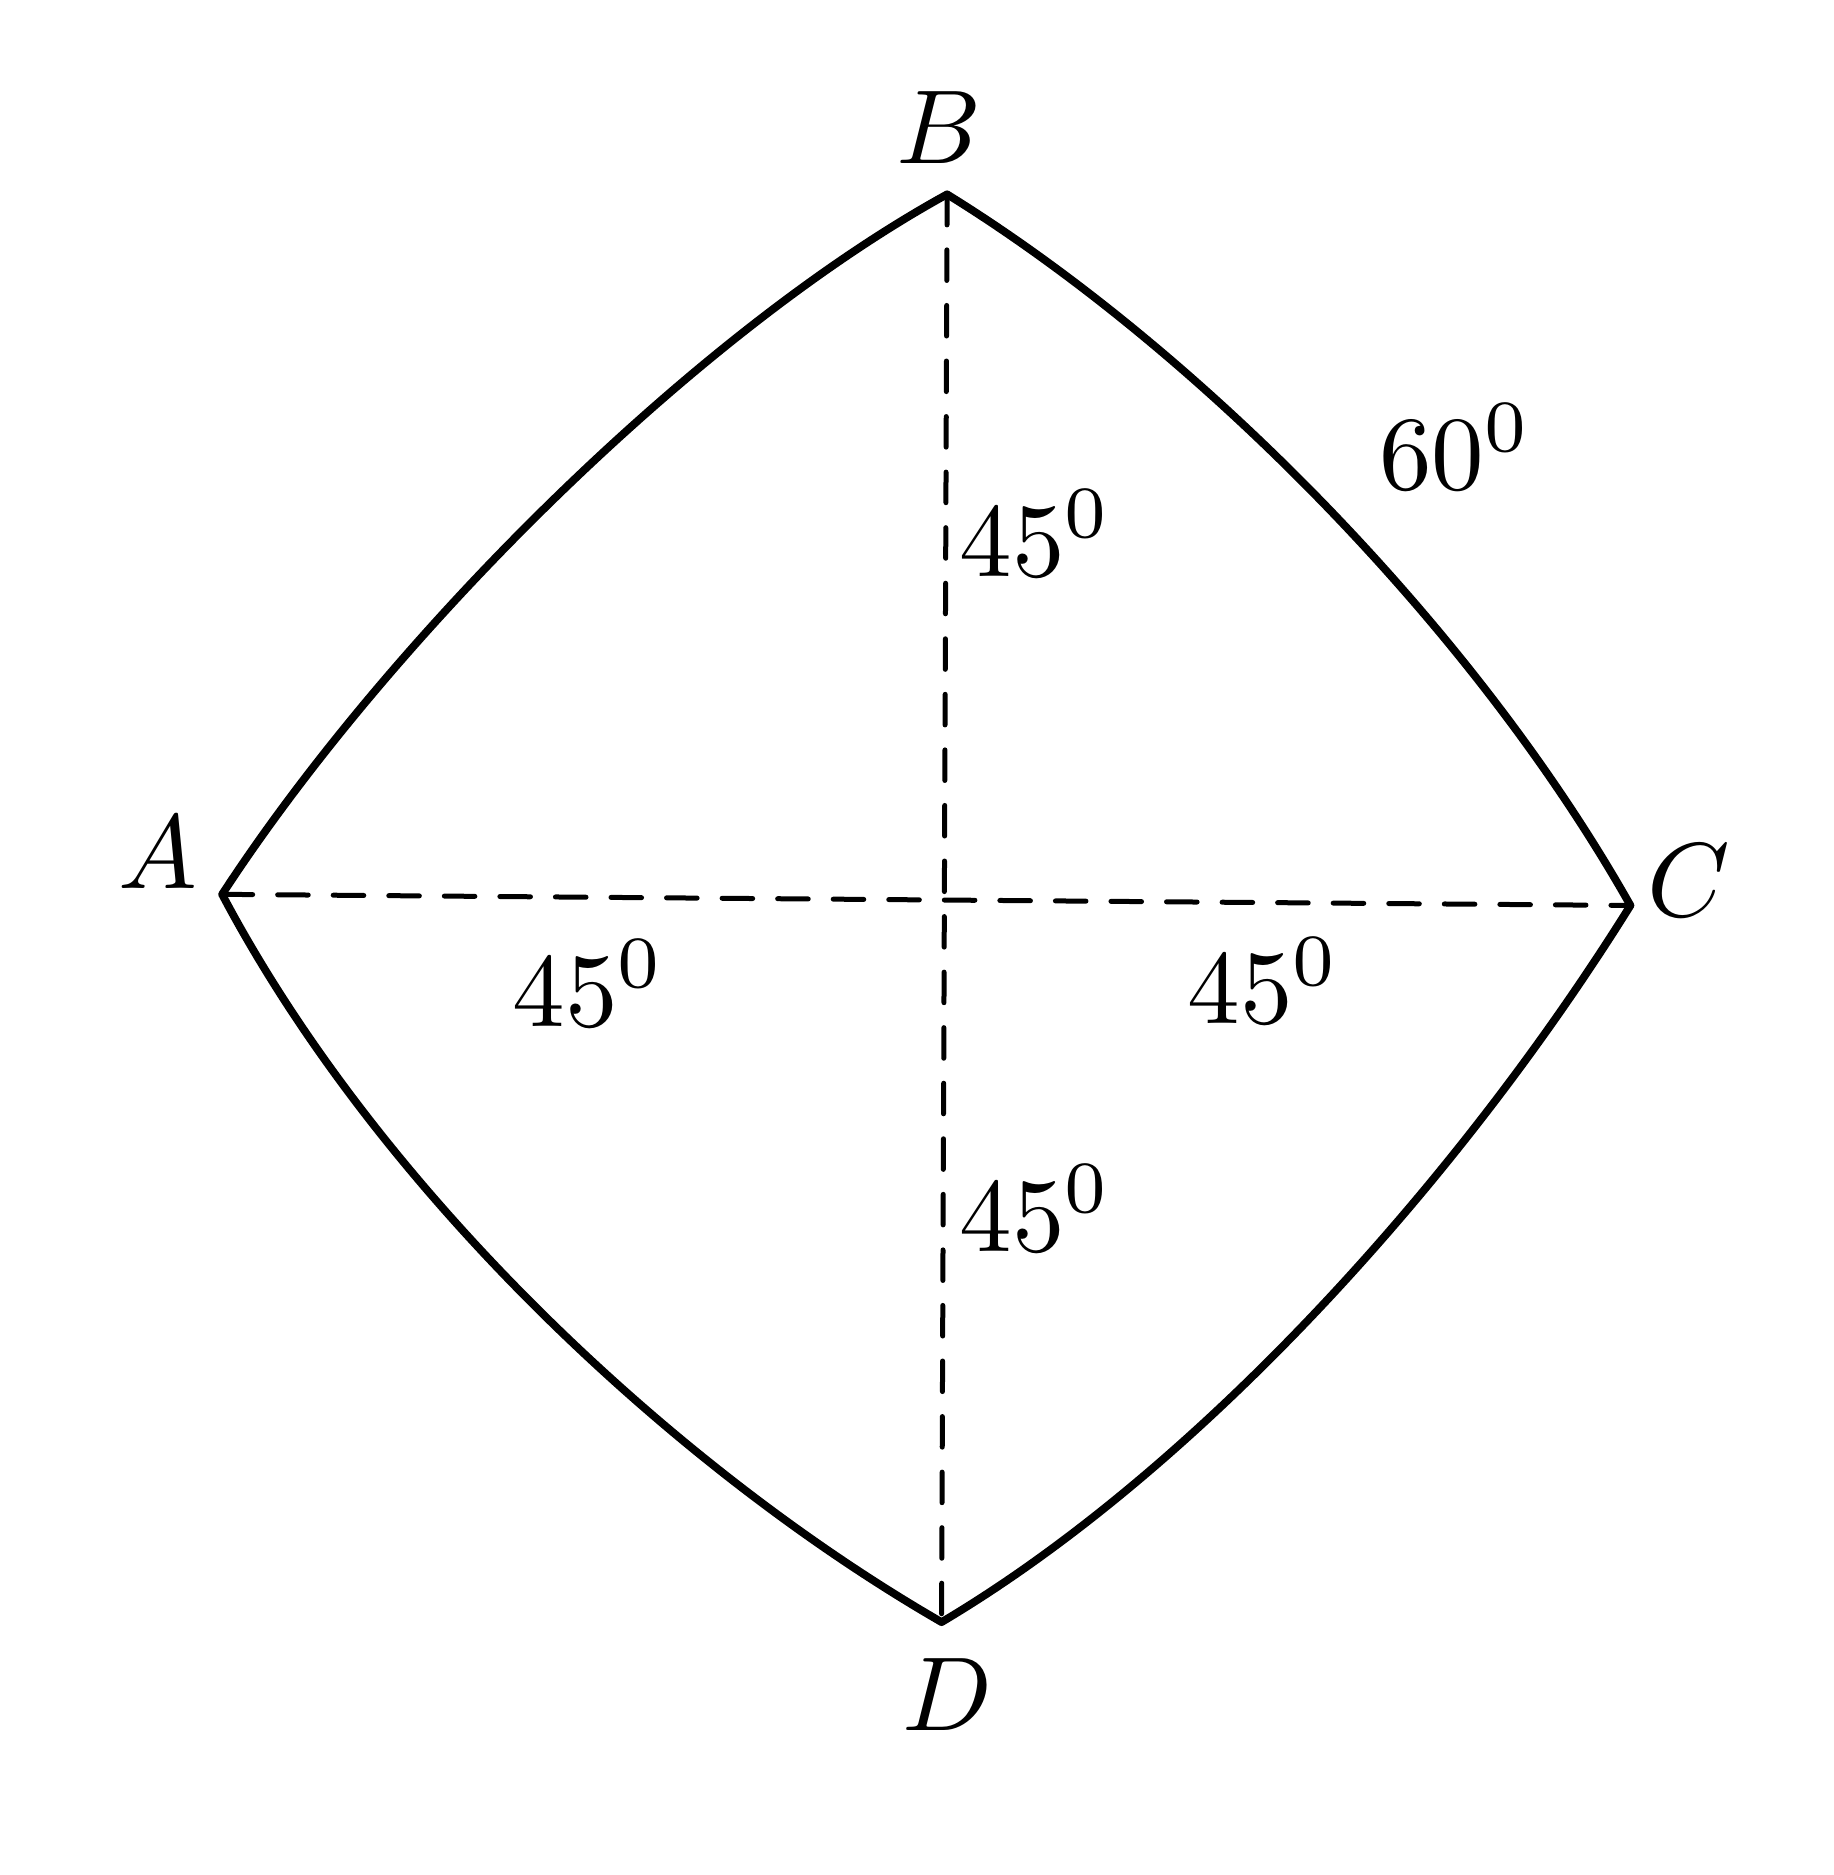
\begin{tikzpicture}[x=1bp,y=-1bp,line cap=round,line join=round]
\path[use as bounding box] (0,0) rectangle (640,655);
\begin{pgfinterruptboundingbox}
\draw[line width=2.8bp] (70,312) .. controls (130,220) and (240,110) .. (331,60) .. controls (420,115) and (520,215) .. (577,316) .. controls (514,417) and (420,520) .. (329,574) .. controls (232,518) and (126,418) .. (70,312);
\draw[line width=1.8bp,dash pattern=on 11bp off 9bp] (70,312) -- (577,316);
\draw[line width=1.8bp,dash pattern=on 11bp off 9bp] (331,60) -- (329,574);
\node[inner sep=0pt,outer sep=0pt] at (47,297) {\scalebox{3.8}{\ensuremath{A}}};
\node[inner sep=0pt,outer sep=0pt] at (328,36) {\scalebox{3.8}{\ensuremath{B}}};
\node[inner sep=0pt,outer sep=0pt] at (598,307) {\scalebox{3.8}{\ensuremath{C}}};
\node[inner sep=0pt,outer sep=0pt] at (331,600) {\scalebox{3.8}{\ensuremath{D}}};
\node[inner sep=0pt,outer sep=0pt] at (363,182) {\scalebox{3.8}{\ensuremath{45^0}}};
\node[inner sep=0pt,outer sep=0pt] at (445,343) {\scalebox{3.8}{\ensuremath{45^0}}};
\node[inner sep=0pt,outer sep=0pt] at (363,425) {\scalebox{3.8}{\ensuremath{45^0}}};
\node[inner sep=0pt,outer sep=0pt] at (202,344) {\scalebox{3.8}{\ensuremath{45^0}}};
\node[inner sep=0pt,outer sep=0pt] at (514,151) {\scalebox{3.8}{\ensuremath{60^0}}};
\end{pgfinterruptboundingbox}
\end{tikzpicture}
}\end{center}
Dritte Ordnung
\[
\alpha\cos PA.\cos PB.\cos PC+\beta\cos PA'.\cos PB'.\cos PC'
\]
wo $A$, $B$, $C$ in einem. $A'$, $B'$, $C'$ in einem andern grössten Kreise liegen und zwar so, dass $AB=BC=CA=A'B'=B'C'=C'A'=120^0$ und beide Kreise einander rechtwinklig schneiden.

Vierte Ordnung: Aggregat dreier Producte aus je vier Cosinus; die drei grössten Kreise schneiden einander unter rechten Winkeln.

Fünfte Ordnung: Aggregat dreier Producte aus je fünf Cosinus. Die drei grössten Kreise schneiden einander in Einem Punkte.

\SourceLeaf{638}
\begin{center}ZUM GEBRAUCH DES COMPARATORS.\end{center}
\begin{center}[1.]\end{center}
Drei in nahe gleichen Entfernungen gesetzte Mikroskope werden successive auf die Theile eines Maassstabes gebracht, die jenen Entfernungen nahe gleich sind.

Die Theilstriche des Maassstabes überschiessen die Sehlinien der Mikro\-skope in diesen successiven Versuchen um
\[
\begin{array}{ccc}
a^0&b^0&c^0\\
a'&b'&c'\\
a''&b''&c''\\
a'''&b'''&c'''\\
&\text{etc.}&
\end{array}
\]
Durch $x^0,y^0,z^0;\ x',y',z';\ x''$ etc. bezeichnen wir die Fehler dieser Grössen. Die Fehlergleichungen sind, wenn
\[
\begin{aligned}
a'-a''-b^0+b''+c^0-c'&=e^0\\
a''-a'''-b'+b'''+c'-c''&=e'
\end{aligned}
\]
u. s. w. gesetzt wird,
\[
\begin{aligned}
x'-x''-y^0+y''+z^0-z'&=e^0\\
x''-x'''-y'+y'''+z'-z''&=e'\ \text{u. s. w.}
\end{aligned}
\]
Hienach haben die plausibelsten Werthe der Fehler die Form
\[
\begin{array}{lll}
x^0=0&y^0=-h^0&z^0=h^0\\
x'=h^0&y'=-h'&z'=h'-h^0\\
x''=h'-h^0&y''=-h''+h^0&z''=h''-h'\\
x'''=h''-h'&y'''=-h'''+h'&z'''=h'''-h''\\
\text{u. s. w.}&&
\end{array}
\]
\SourceLeaf{639}
und die Hülfsgrössen $h^0,h'$ etc. hangen von den Gleichungen ab
\[
\begin{aligned}
6h^0-2h'-h''&=e^0\\
-2h^0+6h'-2h''-h'''&=e'\\
-h^0-2h'+6h''-2h'''-h''''&=e''\\
-h'-2h''+6h'''-2h''''-h^{\mathrm V}&=e'''\\
-h''-2h'''+6h''''-2h^{\mathrm V}-h^{\mathrm {VI}}&=e''''\\
\text{etc.}&
\end{aligned}
\]

\begin{center}[2.]\end{center}
Anordnung der Längen-Comparirungen, um eine Abtheilung eines getheilten Maassstabs in Theilen des ganzen Maassstabs zu bestimmen.

\textit{Beispiel.} Die Theilstriche des Maassstabs waren mit Ziffern von 0 bis 840 bezeichnet. Es sollte die Abtheilung von 0 bis 87 in Theilen des ganzen Maassstabs von 0 bis 840 bestimmt werden. — Zur Abkürzung möge
\[
0\ .\ 87\ .\ 174=\alpha
\]
bedeuten, dass durch Comparirung der Länge 0 bis 87 mit der Länge 87 bis 174 die erstere um $\alpha$ Mikrometertheile grösser als die letztere gefunden worden sei, u. s. f.
\begin{center}Anordnung:\end{center}
\[
\begin{array}{rcrcrcl}
0&.&87&.&174&=&\alpha\\
0&.&174&.&348&=&\beta\\
0&.&348&.&696&=&\gamma\\
840&.&696&.&552&=&\delta\\
840&.&552&.&264&=&\varepsilon\\
0&.&264&.&528&=&\zeta\\
840&.&528&.&216&=&\eta\\
0&.&216&.&432&=&\theta\\
840&.&432&.&24&=&\iota\\
0&.&24&.&48&=&\kappa\\
0&.&48&.&96&=&\lambda\\
0&.&96&.&192&=&\mu\\
0&.&192&.&384&=&\nu\\
0&.&384&.&768&=&\pi\\
840&.&768&.&696&=&\rho
\end{array}
\]

\SourceLeaf{640}
\textit{Berechnung.} Bezeichnet man die ganze Länge des Maassstabs mit $840'$, die gesuchte Länge (von 0 bis 87) mit $87'$, die Länge von 87 bis 174 mit $174'-87'$, u. s. w. so hat man folgende Gleichungen:
\[
\begin{aligned}
2\ .\ 87'-\alpha&=174'\\
2\ .\ 174'-\beta&=348'\\
2\ .\ 348'-\gamma&=696'\\
2\ .\ 696'-840'+\delta&=552'\\
2\ .\ 552'-840'+\varepsilon&=264'\\
2\ .\ 264'-\zeta&=528'\\
2\ .\ 528'-840'+\eta&=216'\\
2\ .\ 216'-\theta&=432'\\
2\ .\ 432'-840'+\iota&=24'\\
2\ .\ 24'-\kappa&=48'\\
2\ .\ 48'-\lambda&=96'\\
2\ .\ 96'-\mu&=192'\\
2\ .\ 192'-\nu&=384'\\
2\ .\ 384'-\pi&=768'\\
2\ .\ 768'-840'+\rho&=696'
\end{aligned}
\]
Hieraus ergibt sich
\[
\begin{aligned}
696'&=-840'+\rho-64.840'+64\iota-256.840'+256\eta-1024.840'\\
&\quad-2\pi-128\theta-512\zeta+1024\varepsilon\\
&\quad-4\nu-2048.840'\\
&\quad-8\mu+2048\delta\\
&\quad-16\lambda+4096.696'\\
&\quad-32\kappa
\end{aligned}
\]
Also ist, wenn $840'=L$, $696'=y$, $87'=z$.
\SourceLeaf{641}
\[
\begin{aligned}
3393L&=4095y+\rho\\
&\qquad-2\pi\\
&\qquad-4\nu\\
&\qquad-8\mu\\
&\qquad-16\lambda\\
&\qquad-32\kappa\\
&\qquad+64\iota\\
&\qquad-128\theta\\
&\qquad+256\eta\\
&\qquad-512\zeta\\
&\qquad+1024\varepsilon\\
&\qquad+2048\delta
\end{aligned}
\]
\[
z=\tfrac18y+\tfrac12\alpha+\tfrac14\beta+\tfrac18\gamma
\]
Hienach wird also der gesuchte Werth von $z=87'$ in Theilen des ganzen Maassstabs $L=840'$ erhalten, wenn das Mikrometer geprüft und dadurch der Werth seiner Theile gleich und in Theilen des Abstands zweier nach obiger Anordnung eingestellter Theilstriche des Maassstabs (z. B. in Theilen der Länge von 87 bis 96) gegeben ist.

\begin{center}ALLGEMEINE FORMELN FÜR DIE WIRKUNG EINES LEUCHTENDEN PUNKTS $P$ AUF EINEN PUNKT $p$.\end{center}
I. Es sei $P$ von $p$ durch eine entweder geschlossene oder unendliche Fläche geschieden, deren offener Theil $s$ heisse, $\mathrm ds$ sei ein Element von $s$, $R,r$ seine Entfernung von $P,p$; $\rho$ eine unbestimmte Normale auf $\mathrm ds$ nach der Seite gerichtet wo $p$ liegt, $\lambda$ eine Wellenlänge, $\dfrac{2\pi i}{\lambda}=\alpha$, $w$ der Winkel zwischen $R$ und $r$: dann wird der Vibrationszustand in $p$ durch
\[
\int\frac{\mathrm ds}{Rr}\left(\frac{\partial R}{\partial\rho}+\frac{\partial r}{\partial\rho}\right)\frac{e^{\alpha(R+r)}}{\sin w}
\]
ausgedrückt, dies Integral durch alle Theile von $s$ erstreckt. Offenbar sind hier $\dfrac{\partial R}{\partial\rho},-\dfrac{\partial r}{\partial\rho}$ die Sinus der Neigungen von $R$ und $r$ gegen $\mathrm ds$.
